\documentclass[10pt,letterpaper]{article}
\usepackage[top=0.85in,left=2.75in,footskip=0.75in,marginparwidth=2in]{geometry}

% use Unicode characters - try changing the option if you run into troubles with special characters (e.g. umlauts)
\usepackage[utf8]{inputenc}

% clean citations
\usepackage{cite}

% hyperref makes references clicky. use \url{www.example.com} or \href{www.example.com}{description} to add a clicky url
\usepackage{nameref,hyperref}

% line numbers
\usepackage[right]{lineno}

% improves typesetting in LaTeX
\usepackage{microtype}
\DisableLigatures[f]{encoding = *, family = * }

% text layout - change as needed
\raggedright
\setlength{\parindent}{0.5cm}
\textwidth 5.25in 
\textheight 8.75in

% use adjustwidth environment to exceed text width (see examples in text)
\usepackage{changepage}

% adjust caption style
\usepackage[aboveskip=1pt,labelfont=bf,labelsep=period,singlelinecheck=off]{caption}

% remove brackets from references
\makeatletter
\renewcommand{\@biblabel}[1]{\quad#1.}
\makeatother

% headrule, footrule and page numbers
\usepackage{lastpage,fancyhdr,graphicx}
\usepackage{epstopdf}
\pagestyle{myheadings}
\pagestyle{fancy}
\fancyhf{}
\rfoot{\thepage/\pageref{LastPage}}
\renewcommand{\footrule}{\hrule height 2pt \vspace{2mm}}
\fancyheadoffset[L]{2.25in}
\fancyfootoffset[L]{2.25in}

% use \textcolor{color}{text} for colored text (e.g. highlight to-do areas)
\usepackage{color}

% define custom colors (this one is for figure captions)
\definecolor{Gray}{gray}{.25}

% this is required to include graphics
\usepackage{graphicx}

% use if you want to put caption to the side of the figure - see example in text
\usepackage{sidecap}

% use for have text wrap around figures
\usepackage{wrapfig}
\usepackage[pscoord]{eso-pic}
\usepackage[fulladjust]{marginnote}
\reversemarginpar

% document begins here
\begin{document}
\vspace*{0.35in}

% title goes here:
\begin{flushleft}
{\Large
\textbf\newline{Maize Local Adaptation to Low Soil Phosphorus Availabilty: \\ Environmental Genome Wide Association.}
}
\newline
% authors go here:
\\
Fausto Villafrade Rodriguez Zapata\textsuperscript{1}.
\\
\bigskip
\bf{1} LANGEBIO, CINVESTAV.
\\
\bigskip
* fausto.rodriguez@cinvestav.mx

\end{flushleft}

\section*{Abstract}
Phosphorus starving response (PSR) is a physiological and developmental shift experienced by plants when confronted to low phosphorus availability. Assuming that PSR is a local adaptation, I expect differences in allelic frequencies between populations grown on habitats with distinguishing soil phosphorus availability. Consequently I also expect evidence of divergent selection on loci related to PSR. Here I use a reverse ecology approach in order to dissect PSR genetic architecture in a wider context of highland maize adaptation. First I build soilP, an R package that allows the user to retrieve soil phosphorus retention potential values. With this retention potential as a proxy for phosphorus availability I perfrom environmental GWAS on two datasets of georeferenced genotypes, one for \textit{Zea mays} another for \textit{Arabidopsis thaliana}. I find biologically meaningful hits for protein coding genes in both species regarding  macronutrient and lipid metabolism; and hormone biosynthesis and signal transduction. However, differences in the identity of the association hits are congruent with the evolution of different PSR in maize and \textit{Arabidopsis}. I further discuss confounding effects of population strucucture and demographic history, proposing Qst/Fst analysis  and QTL mapping on biparental an other seggregating populations as the next logical steps of this reasearch.


% now start line numbers
\linenumbers

% the * after section prevents numbering
\section*{Introduction}

Phosphorus is a limiting nutrient for plant growth because it is essential for metabolism and has both, high plant demand and low soil availability \cite{Agren:2012kg}. For optimal growth, plants can increase inorganic phosphorus (Pi) concentration by a factor of 1000, from around 10 uM in soil solution, to 10 mM in the symplast \cite{Lambers:2015ut,Schachtman:1998vv}. Soil mineralogy and pH determine the amount of biologically available Pi. In acid conditions phosphates precipitate in the presence of aluminum and iron cations, while in basic conditions Pi forms insoluble salts of calcium and magnesium. This chemical reactivity restricts soil P bioavailability as Al, Fe an Ca are the 1st, 2nd, and 3rd most abundant metals in earth's crust, mostly present as oxides \cite{Rudnick:QE13oOmz}, e.g. in clay minerals. Therefore, typical basic and acid soils have chemical compositions that promote phosphate precipitation. First, because alkalinity in soils is often, but not always, due the presence of calcium carbonates. Second, because acid soils at first solubilize Al and Fe cations that are, in turn, taken out of the solution by phophate anions. In addition to precipitation, phosphorus becomes less available to plants due to sorption into minerals composed of oxides and hydroxides of Al, Fe and Mn at acidic pH, and to a lesser extent over calcium compounds in alkaline pH \cite{Prasad:2016ca}. Not only bivalent cations in solution push chemical equilibrium towards precipitated phosphates in both types of soils, but also those same cations, this time as part of mineral surfaces, adsorb an additional Pi fraction. 

Different soil phosphorus compounds can be sorted into separate pools according their availability for direct plant use. The most readily available form for plants is Pi in aqueous solution. Next, is the phosphorus in organic compounds, such as nucleotides, phospholipids, phosphorilated sugars and proteins, that can be converted into phosphates by enzymatic activity. After this, the non-occluded P fraction corresponds to phosphate adsorbed to the surfaces of iron and aluminium oxides and hydrous oxides and CaCO3 \cite{WALKER19761}. One step less available is the occluded P fraction, that is, phosphate physically encapsulated or surrounded by secondary minerals, such as Fe, Al and Mn oxyhydroxides \cite{Yang:2013ft,Filipelli:6Zj8wyph} by coprecipitation or diffusive penetration \cite{WALKER19761}. Thus the labile, i.e. more bioavailable \cite{Yang:2013ft}, phosphorus pool includes phosphate ions in solution as well as P incorporated in soil organic matter, and to a lesser degree the non-occluded P fraction. The refractory forms, which are not readily bioavailable, include P in non-weathered apatite minerals and the ocludded P fraction \cite{Filipelli:6Zj8wyph}. 

In experimental conditions added high or normal Pi concentrations in nutrient solution range from 15 uM to 0.1 mM, depending on the subject species \cite{Scheible:2015hxa}. However lower realized concentrations are expected given phosphate precipitation in presence of calcium ions, that are usually part of the solution. Pi concentrations 0.3 to 5 uM in soil solution, could be considered low if they do not support optimal plant growth \cite{Scheible:2015hxa,Schachtman:1998vv}, thus depending on subject species as well. Unfertilized soils rarely release P fast enough to support the high growth rates of crop plant species \cite{Schachtman:1998vv}.

When confronted with Pi scarcity, plants present biochemical, physiological and developmental adjustments, collectively known as phosphate starving response (PSR), that can improve aquisition, reallocation, mobilization and, in general, phosphorus use efficiency \cite{Scheible:2015hxa}. Pi starvation results in a shift in the developmental program that can increase the fitness of the plant \cite{Peret:2011jd}, therefore this shift can be conceived as adaptive, not only in the ontological but also in the evolutionary sense.

The strict criterion for local adaptation is that a population must have higher fitness at its native site than any other population introduced to that site \cite{Savolainen:2013df}. Local adaptation results in higher fitness  of a population in a local environment, relative to populations coming from different habitats \cite{Kawecki:2004hx}. It is both the observed pattern and the process dependent on divergent selection, the allele frequency change in the populations in response to selection that varies geographically \cite{Tiffin:2014ft}. Evolutionary forces against local adaptation include gene flow, migration and  mutation, because  they act contrary to genetic differentiation of the populations. In contrast genetic drift causes differentiation in allele frequencies that is not necessarily adaptive, and is thus a confounding factor when studying the genetic basis of local adaptation \cite{Kawecki:2004hx}.



"difference between non-occluded and occluded P is by no means absolute but non-occluded P is believed to represent phosphate ions sorbed at the surfaces of iron and aluminium oxides and hydrous oxides and CaCO3, and occluded P refers to phosphate ions present within the matrices of retaining components following diffusive penetration" \cite{WALKER19761}


"Pierre and Parker (1927) measured an average Pi concentration in the soil solution of 3 uM in a study of 21 different soils from the South and Middle West of the USA (range: <0.6 to 11 uM), far lower than the intracellular Pi concentrations (5–20 mM) required for optimal crop growth (Fang et al., 2009; Vance et al., 2003)."\cite{Lambers:2015ut}. "The form of P most readily accessed by plants is Pi, the concentration of which rarely exceeds 10uM in soil solutions (Bieleski, 1973)" \cite{Schachtman:1998vv} "Cytoplasmic Pi is maintained at constant concentrations (5–10 mm), more or less independently of external Pi concentrations, except under severe P depletion (Lee et al., 1990; Lee and Ratcliffe, 1993; Mimura, 1995). " \cite{Schachtman:1998vv} "Concentrations of Pi in the xylem range from 1 mm in Pi-starved plants to 7 mm in plants grown in solutions containing 125  m Pi (Mimura et al., 1996). " \cite{Schachtman:1998vv}.

"The phosphorus in soils is present in a variety of forms, and the distribution of P between these forms dramatically changes with time and soil development. The forms of soil P can be grouped into refractory (not readily bioavailable) and labile (readily bioavailable). The refractory forms include P in apatite minerals and P coprecipitated with and/or adsorbed onto iron and manganese oxyhydroxides (termed occluded P). The reducible oxyhydroxides have large binding capacities for phosphate, due to their immense surface area and numerous delocalized positively charged sites (e.g., Smeck 1985; Froelich 1988). The labile forms include P in the soil pore spaces (as dissolved phosphate ion) and adsorbed onto the soil particle surfaces (these forms are termed nonoccluded P), as well as P incorporated in soil organic matter. On a newly exposed lithic surface, nearly all of the P is present as P in apatite. With time and soil development, however, P is increasingly released from this form and incorporated in the others (Figure 1.2)." \cite{Filipelli:6Zj8wyph}

"Although the total P content of soils can be large, in most soils, only a small fraction is available for bioLogical utilization because it is either bound in incompletely weathered mineral particles, adsorbed on mineral surfaces,or, over the time of soil formation, made unavailable by secondary mineral formation (occluded)." \cite{Yang:2013ft}

"Chronosequence studies show decreasing total P content during pedogenesis, while available P first increases from weathering and then decreases as a result of various soil processes" \cite{Yang:2013ft} "Gelisol, Histosol, Andisol are not considered in this study since they are con- sidered as special soil orders that have unique genetic prop- erties unrelated to the stage of soil development." \cite{Yang:2013ft}

Adaptation to low soil P availability.

"plants respond to P-limitation with a multifaceted set of morphological, physiological, metabolic, biochemical, and molecular changes, collectively called the PSR, which may improve P-acquisition, P-reallocation and remobilisation, and overall P-use efficiency"  \cite{Lambers:2015fx}
"Adaptive P-starvation responses of vascular plants. Plants have evolved a wide range of adaptations to Pi-limitation that include an expansion of their soil exploration capacity (e.g. through root system architecture (RSA) changes or establishment of mycorrhizal symbioses), improved Pi acquisition from otherwise inaccessible sources of soil P (e.g. root secretion of purple acid phosphatases, ribonucleases, phosphodiesterases, and excretion of organic acids (OA)), enhanced Pi transport capacity (e.g. upregulation of high-affi nity Pi transporters), and the protection of plant metabolism from deleterious effects of P-starvation (e.g. storage and accumulation of secondary metabolites such as anthocyanins). The systemic signals underlying the PSRs are delivered from the root and shoot tissues through the xylem (red arrowheads) and phloem (yellow arrowheads) streams, respectively. LR, lateral root; RH, root hair; PR, primary root." \cite{Lambers:2015fx}
 Responses to phosphorus starvation include increase of soil P absortion/uptake/acquisition, mobilization from storage old leaves, recycling, diminished Pi related metabolism, increased association with mycorrhyzal fungi \cite{Lambers:2015fx}, root modification \cite{Lambers:2015fx}, hormone signanling \cite{Lambers:2015fx}. 


Proof of local adaptation. Local adaptation: adaptation in response to selection that varies geographically \cite{Tiffin:2014ft}. Coupling of isolation by distance and isolation by environment, relative contribution of geography and environment, redundancy analysis \cite{Lasky:2015hp}, to genetic structure \cite{Tiffin:2014ft}.Evidence consistency. Allele association. "predict the performance of genotypes on the basis of candidate genes identified through climate associations:  applied this to predict performance in a common garden" \cite{Tiffin:2014ft,Lasky:2015hp}  "Therefore, the existence of a pattern of local adaptation despite gene flow certifies to the strength of natural selection imposed by particular environmental factors" \cite{Kawecki:2004hx}. "the strict criterion for local adaptation is that a population must have higher fitness at its native site than any other population introduced to that site" \cite{Savolainen:2013df}. Local adpatation results in higher fitness  of a population in a local environment, relative to populations of different habitat.It is both the observed pattern and the process dependent on divergent selection. Evolutionar against local adaptation include gene flow, migration, mutation. Genetic drift causes diffrentiation in allele frequencies that are not necesaraly adaptative. 
"Protected polymorphism in a heterogeneous environment may be maintained even if dispersal results in complete mixing of the gene pool. However, in such a case demes will not differentiate genetically, i.e. there will be no local adaptation. Thus,restricted gene flow is a pre-requisite for local adaptation." (What does this mean?) \cite{Kawecki:2004hx} 
"Local adaptation should be manifested in improved fitness of each deme in its own habitat." \cite{Kawecki:2004hx}  "For local adaptation to occur, high fit- ness in one environment must have a cost in the other environment, and migration should not overwhelm the effect of local selection" \cite{Savolainen:2013df}."When selection for local adaptation takes place with ongoing gene flow, evolution towards fewer loci with larger-effect-size alleles is expected" \cite{Savolainen:2013df}."In one well- studied case, differential predation by owls is likely to maintain coat colour differences of beach mice between environments despite extensive migration92. In this migration–selection balance situation, large-effect muta- tions in the cis-regulatory region of the Agouti locus and in the coding region of the Mcr1 locus account for much of the coat colour variation." \cite{Savolainen:2013df}. "we would like to reiterate that local adaptation as defined above is not a property of individual populations, but of a set of demes (i.e. a metapopulation)." \cite{Kawecki:2004hx} "Demonstrating a pattern consistent with local adaptation certifies to the power of divergent selection relative to gene flow and other evolutionary processes." \cite{Kawecki:2004hx} "Traits mediating local adaptation should show genetically based phenotypic differences between demes evolved in different habitats, the phenotype being understood broadly to include physiological and biochemical characteristics and patterns of gene expression. However, not all genetically based phenotypic differences between demes must be adaptive. Instead they may represent the costs of adaptive traits, mediated by pleiotropic effects of underlying genes. They may also be because of genetic hitchhiking of genes linked to those favoured by divergent selection. Finally, such differences may be produced by processes not related to local adaptation (such as drift or evolution of alternative coadapted gene combinations)." \cite{Kawecki:2004hx} "how much additive genetic variation for this trait exists and how is it distributed within vs. among demes? The former indicates the ability of the trait to respond to selection (for estimation see Falconer  Mackay 1996; Lynch Walsh 1998, part III). The latter, which can be quantified as Qst (Merila  Crnokrak 2001; McKay Latta 2002), measures the degree of genetic differentiation of quantitative traits between populations. Traits under strongest divergent selection are expected to have the highest Qst, which is another way of identifying traits mediating local adaptation." \cite{Kawecki:2004hx} 


Reciprocal transplant and common garden experiments. 
"Such reciprocal transplants will often be impossible for practical, ethical or legal reasons." \cite{Tiffin:2014ft,Kawecki:2004hx} (check again tiffin). "The downside is that local adaptation to habitat differences neglected in the experiment may confound the results." \cite{Kawecki:2004hx} 
"Note finally that, although common garden experiments are closely related to reciprocal transplant experiments (which aim at testing local adaptation by showing that the average fitness of local individuals is higher than the average fitness of aliens, see for example Agren and Schemske, 2012), there are important philosophical and practical differences between the two types of experiments.The difference is that reciprocal transplants are designed to prove local adaptation, whereas common gardens are designed to study the genetic bases of traits, regardless of whether they are adaptive or not. In practice, reciprocal transplants will typically create a differential survival, because the locals will survive better. This will be a confounding effect during the quantitative genetic analysis, because only the phenotypes of ‘fit’ individuals are available. Common gardens, by contrast, are often designed to be ‘softer’ on the individuals. Nevertheless, most of the elements in this article regarding common garden experiments can also be applied to reciprocal transplants, especially if one is interested in applying them to survival or some other measure of fitness." \cite{deVillemereuil:2015ge}


Population - Population structure.
Population definition. "The questions that can be addressed in local adaptation studies crucially depend on experimental design, and especially on the choice of populations." \cite{Savolainen:2013df} "to map genes that are related to local adaptation, by definition, genetically differentiated popu- lations need to be studied." \cite{Savolainen:2013df}. "Combining association studies with QTL mapping105 or artificial multi-accession crosses105,111 allows the consideration of many parents and seems to be promising for increasing mapping accuracy and resolving confounding problems, as demonstrated by a detailed analysis of flowering time in maize"\cite{Savolainen:2013df}. "a reproductive community of individuals who share in a common gene pool" \cite{DOBZHANSKY:1955uz,Dobzhansky:1950}. "Mendelian popula- tions are usually organized into systems of various orders.The species is, in sexual and cross-fertilizing organisms, the most inclusive Mendelian popula- tion." \cite{DOBZHANSKY:1955uz}  The infra-specific Mendelian populations main- tain more or less distinct gene pools because they are, as a rule, separated in space." \cite{DOBZHANSKY:1955uz} "the marriage regulation by custom, language, re- ligion, class and caste, economic status, and occu- pation has introduced new population sub-divisions, which may be on their way towards superseding the geographic divisions. "  \cite{DOBZHANSKY:1955uz} "individuals and genotypes in a Mendelian population are components of an organismic sys- tem; they are multiply related through common descent as well as through the bonds of mating and parentage."\cite{DOBZHANSKY:1955uz}  "Naive approaches to population definition "geography-based assignment might not validly capture the selective environments, and ignorance of demography can greatly skew estimates of the loci under selection and the strength of that selection" \cite{Tiffin:2014ft}. On the other extreme "methods for understanding how selection shapes within-species patterns of variation are highly depen- dent on nonequilibrium population histories. In order to ac- count for this reliance, researchers either take a predefined fraction of loci in the tails of a distribution as the number affected by selection, or assume that a nonequilibrium history explains the majority of the data by fitting a highly embellished model of demography in order to erase all signs of outliers." \cite{Kern:2018db}

"landraces are extensively used by agronomists, who recognize them as stable and discriminatory categories for the classification of samples." \cite{CalduPrimo:2017eh} "Maize landraces can be defined as dynamic populations with a historical origin and distinct identity, and which are often genetically diverse, locally adapted, and associated with a set of farmers’ practices of seed selection and field management as well as with traditional knowledge (Camacho-Villa et al., 2015)" \cite{CalduPrimo:2017eh} "Clustering by Landrace is Achieved Only with High FST SNPs"\cite{CalduPrimo:2017eh} "Crop landraces represent a readily available resource to address these issues, because they are cultivated material already adapted to low-input agriculture, marginal lands, or stressful environments. For instance, maize landraces have an evolved adaptability to a wider range of environmental conditions than teosinte" \cite{GiandomenicoCorrado:2017bk} "Similarly, a rice variety originating from regions with poor soil (e.g., phosphorus-deficient lowlands) was used to isolate the phosphorus-starvation tolerance 1 (PSTOL1) gene, which is absent in modern varieties" \cite{GiandomenicoCorrado:2017bk}
GWAS.


GWAS Maize, Arabidopsis.


In the introduction you will see an example of text wrapping around the figure with a figure caption on the margin (Fig. \ref{fig1}). This is done by combining the \verb!wrapfigure! with % avoid blank space here 
\marginpar{
\vspace{.7cm} % adjust vertical position relative to text with \vspace{} - note that you can enter negative numbers to move margin caption up
\color{Gray} % this gives caption a grey color to set it apart from text body
\textbf{Figure \ref{fig1}. Example of a margin caption.} % note that \ref{fig1} refers to the corresponding wrapfigure
Setting up your figure + caption like this looks fancy and does not disrupt the flow of the text. But it requires more manual adjustments (position, spacing, labeling) compared to using standard \LaTeX figure environments.
}
\begin{wrapfigure}[19]{l}{75mm}
% the number in [] of wrapfigure is optional and gives the number of text lines that should be wrapped around the text. Adjust according to your figures height
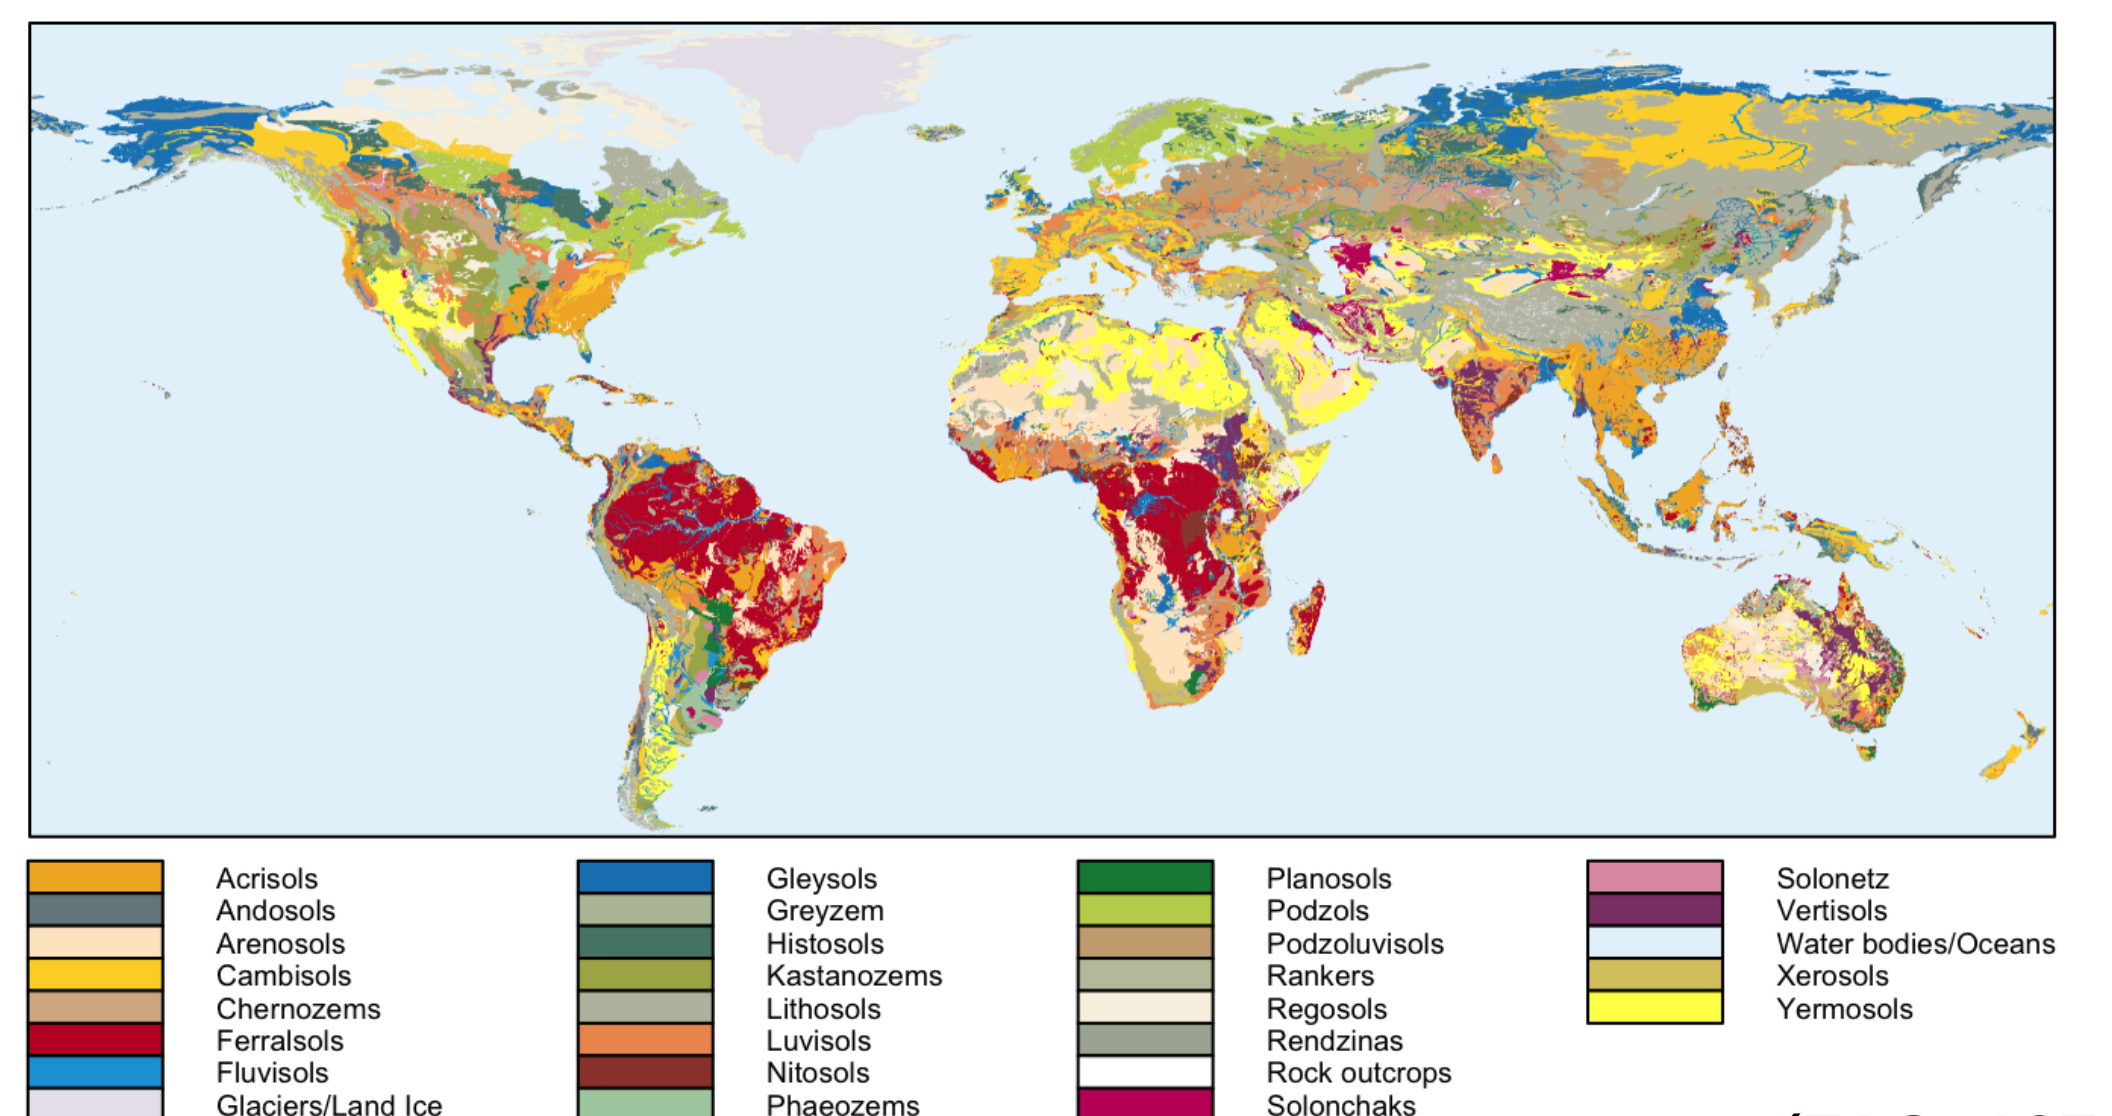
\includegraphics[width=75mm]{fig1.pdf}
\captionsetup{labelformat=empty} % makes sure dummy caption is blank
\caption{} % add dummy caption - otherwise \label won't work and figure numbering will not count up
\label{fig1} % use \ref{fig1} to reference to this figure
\end{wrapfigure} % avoid blank space here
the \verb!marginnote! environment. Please note that in this case the figure (\verb!wrapfigure!) and the figure caption (\verb!marginpar!) have to be separated as you can tell from the code. The \verb!wrapfigure! environment can be a bit tricky when it comes to text formatting. Thus some general hints: (a) try to avoid line breaks in the code as this may result in weird formatting around the figure, (b) the figure should not span multiple headlines (sections) and (c) if you encounter problems with the line break right after the \verb!wrapfigure! try using \verb!\mbox{}! to prevent premature line breaks (\mbox{see example in code}). As stated in the figure caption, setting up figures this way requires a bit more manual adjustments but it makes figures blend in nicely without interrupting flow of text.

\section*{Materials and Methods}

\subsection*{Tables.} 

In this section you will find an example of a table using the \verb!table! plus the \verb!adjustwidth! environment and should give you a minimal example for tables in \LaTeX (Table \ref{tab1}).

\begin{table}[!ht]
\begin{adjustwidth}{-1.5in}{0in} % comment out/remove adjustwidth environment if table fits in text column.
\centering
\caption{{\bf Example Table.} This table demonstrates how to use the  adjustwidth environment if you need that tad bit of extra width for your figures or tables.}
\begin{tabular}{|l|l|l|l|l|l|l|}
\hline
\multicolumn{4}{|l|}{\bf Heading 1} & \multicolumn{3}{|l|}{\bf Heading 2}\\ \hline
cell 1 - row 1 & cell 2 - row 1 & cell 3 - row 1 & cell 4 - row 1 & cell 5 - row 1 & cell 6 - row 1 & cell 7 - row 1 \\ \hline
cell 1 - row 2 & cell 2 - row 2 & cell 3 - row 2 & cell 4 - row 2 & cell 5 - row 2 & cell 6 - row 2 & cell 7 - row 2 \\ \hline
cell 1 - row 3 & cell 2 - row 3 & cell 3 - row 3 & cell 4 - row 3 & cell 5 - row 3 & cell 6 - row 3 & cell 7 - row 3 \\ \hline
\end{tabular}
\label{tab1}
\end{adjustwidth}
\end{table}

\paragraph{Paragraph.}
Instead of adding more and more subsections you can use the \verb!\paragraph{}! command to give structure to your manuscript.

\subsection*{Formulas.}
For mathematical formulas you should use the math environment. See this example:

\begin{center}
$f(A_{ik},A_{jk}) = min(A_{ik},A_{jk}) - C_{1} max(A_{ik},A_{jk}) e^{-C_{2}min(A_{ik},A_{jk})}$
\end{center}

% newpage forces a page break if you want to clearly separate materials from results
\newpage

\section*{Results}
\subsection*{Standard floating figures.}
Figure \ref{fig2} is wrapped into a standard floating environment. That means that \LaTeX will determine the exact placement of the figure. Even though you can state preferences (see code) it can be tricky to get the right placement - especially when working on very tight manuscripts. If you want exact placement, add \verb!\usepackage{float}! to this file's header and use [H] in the figure environment's placement options.


\begin{figure}[ht] %s state preferences regarding figure placement here

% use to correct figure counter if necessary
%\renewcommand{\thefigure}{2}

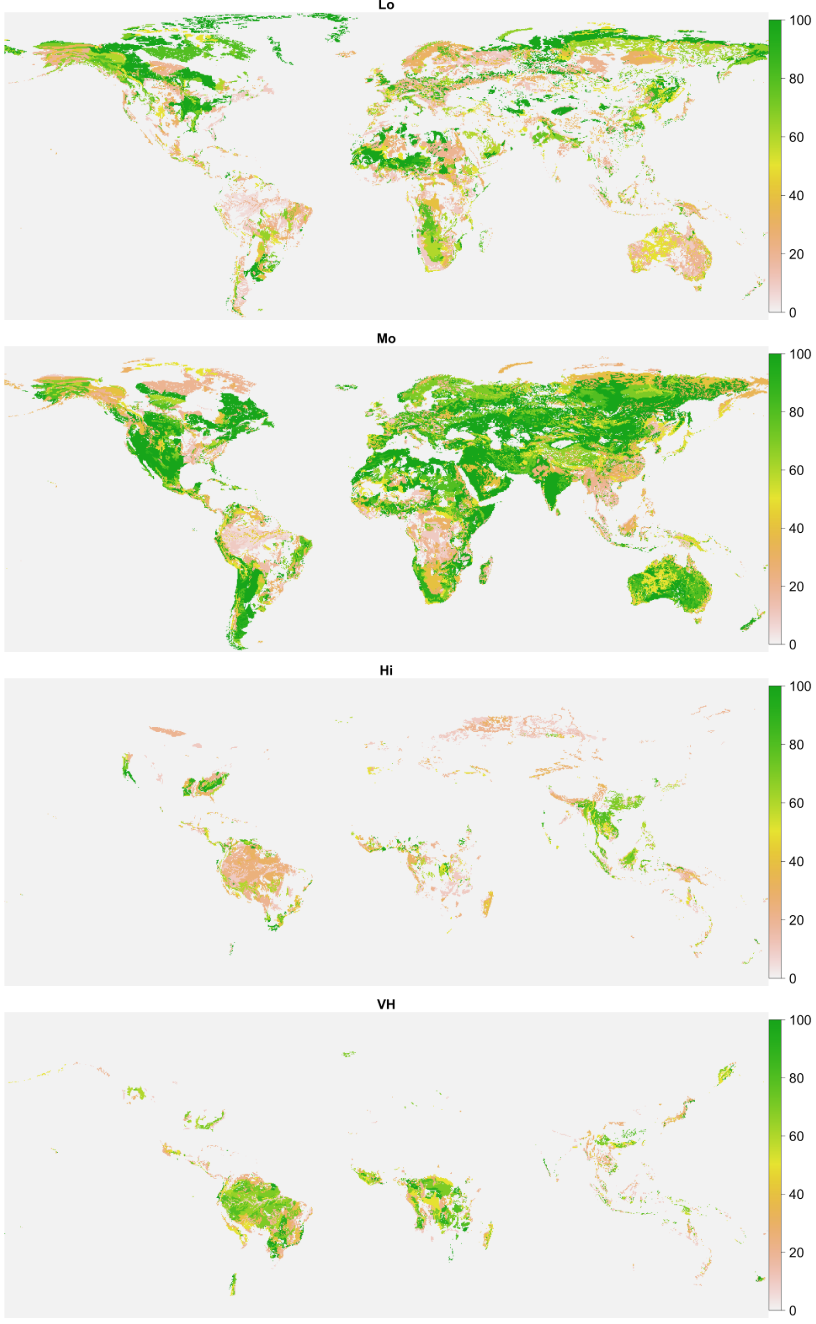
\includegraphics[width=\textwidth]{fig2.pdf}

\caption{\color{Gray} \textbf{Example of a standard floating figure}. \textbf{A-F}, This figure is wrapped into the standard floating environment.}

\label{fig2} % \label works only AFTER \caption within figure environment

\end{figure}

\subsection*{Page break in figures.}
The standard floating figures in \LaTeX do not cope well with page breaks which can make it difficult to fit in large figures. One way to deal with this is to separate figure and caption but \verb!\caption{}! might still give troubles at page breaks. Figure 3 demonstrates a way to manually set up figure and caption such that it continues onto the next page.
\vspace{.5cm} % set vertical space between text and figure
\begin{adjustwidth}{-2in}{0in}
\begin{flushright}
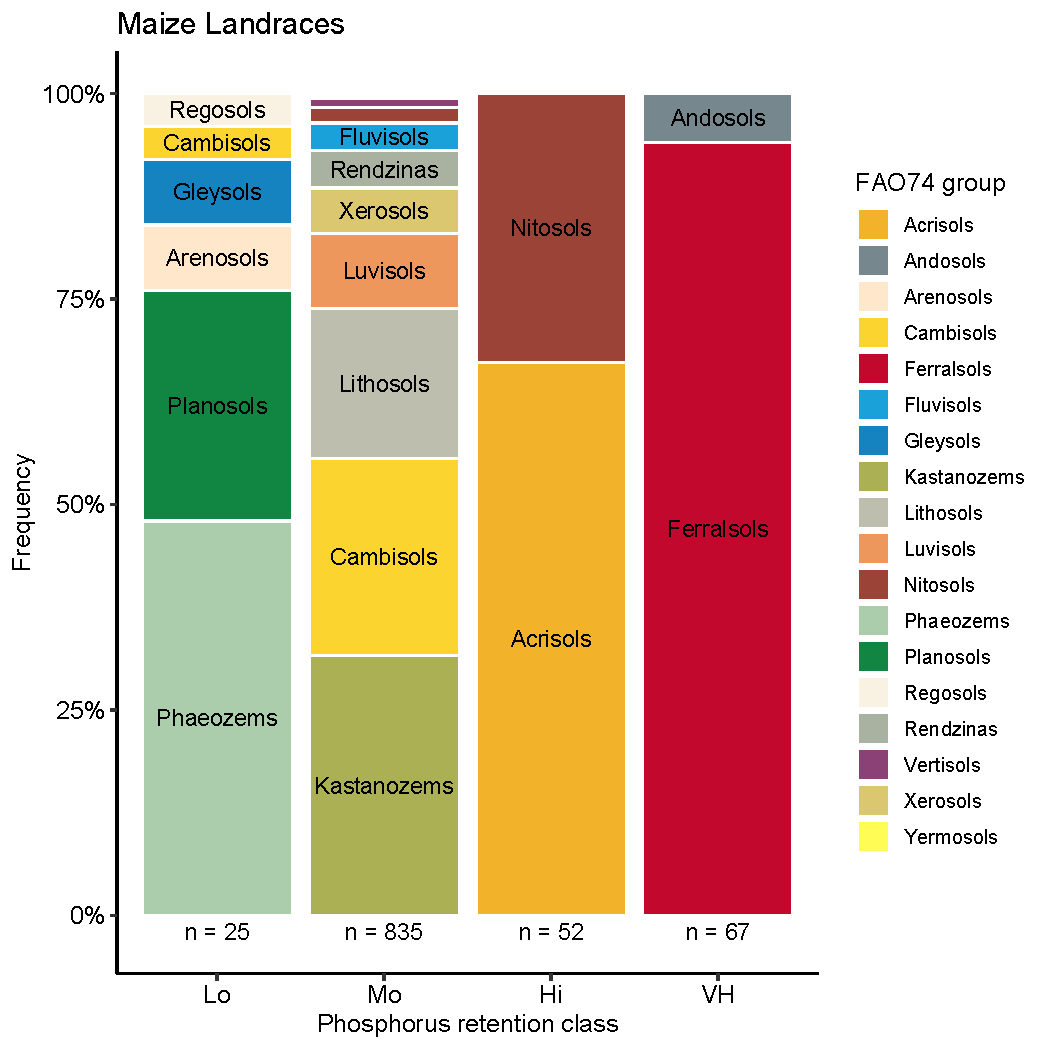
\includegraphics[width=163mm]{fig3.pdf}
\end{flushright}
\justify 
\color{Gray}
\textbf {Figure 3. Example of a wide figure with multi-page caption.}
\textbf{A}, Proin lectus ex, venenatis vel ornare eget, hendrerit tempus justo. Pellentesque molestie purus sed pretium tincidunt. Curabitur facilisis, orci vitae mollis fringilla, elit erat fermentum justo, nec luctus nunc sapien vel dolor. Cras enim justo, ullamcorper ut commodo at, posuere et ex. Fusce cursus sapien id augue maximus convallis. Praesent egestas massa in enim volutpat varius. In aliquam turpis urna, at elementum turpis eleifend at. \textbf{B}, Proin risus erat, tincidunt quis massa non, sollicitudin congue metus. Aliquam quis magna vulputate, posuere est eu, tempor nisi. Cras gravida tempus felis, vitae lacinia lacus volutpat quis. Pellentesque et eros eu mi suscipit tempus. Proin in augue scelerisque. \textbf{C}, Donec a tempor tortor, et dignissim enim. Cras in ipsum sed velit bibendum imperdiet. Aenean aliquet mauris maximus, sodales ligula sit amet, placerat felis. In tristique nisi eu risus rutrum, ac lacinia lorem cursus. Nunc eget condimentum purus. Maecenas imperdiet nisl eu accumsan gravida. \textbf{D}, Nullam tincidunt, magna sed auctor ultrices, leo mi eleifend velit, quis varius ex diam non tellus. Nam tincidunt vehicula turpis, ut euismod turpis elementum vel.
\end{adjustwidth}


%\clearpage makes sure that all above content is printed at this point and does not invade into the upcoming content
%\clearpage

\section*{Discussion}
\subsection*{Subsection heading.}

Lorem ipsum dolor sit amet, consectetur adipiscing elit. Aliquam bibendum finibus diam, gravida sagittis lorem gravida vitae. Interdum et malesuada fames ac ante ipsum primis in faucibus. Nulla in diam tristique ante posuere tristique. Donec interdum purus sit amet nisl accumsan consectetur. Fusce aliquet libero mi, quis ornare dolor congue ullamcorper. Nulla nulla urna, molestie in urna sed, lacinia volutpat eros. Ut mi libero, elementum scelerisque ipsum vel, hendrerit fermentum turpis. Aliquam sit amet leo sodales, egestas augue id, fermentum nulla. Aenean vel cursus ante, et pellentesque eros. Nulla ac neque nec justo posuere commodo sit amet sit amet justo. Aliquam tincidunt tempor ex nec tincidunt. In ullamcorper vehicula lobortis. 

%\clearpage

\section*{Supporting Information}
If you intend to keep supporting files separately you can do so and just provide figure captions here. Optionally make clicky links to the online file using \verb!\href{url}{description}!.

%These commands reset the figure counter and add "S" to the figure caption (e.g. "Figure S1"). This is in case you want to add actual figures and not just captions.
\setcounter{figure}{0}
\renewcommand{\thefigure}{S\arabic{figure}}

% You can use the \nameref{label} command to cite supporting items in the text.
\subsection*{S1 Figure}
\label{example_label}
{\bf Caption of Figure S1.} \textbf{A}, If you want to reference supporting figures in the text, use the \verb!\nameref{}!. command. This will reference the section's heading: \nameref{example_label}.

\subsection*{S2 Video}
\label{example_video}
{\bf Example Video.} Use \href{www.youtube.com}{clicky links} to the online sources of the files.

%\clearpage

\section*{Acknowledgments}
We thank just about everybody.

\nolinenumbers

%This is where your bibliography is generated. Make sure that your .bib file is actually called library.bib
\bibliography{library}

%This defines the bibliographies style. Search online for a list of available styles.
\bibliographystyle{abbrv}

\end{document}

